\pagestyle{fancy}
\normalsize
\linespread{1.5}\selectfont
\label{mark:chapter2}\chapter{背景知识}
\addtocontents{los}{\protect\addvspace{10pt}}

\section{重组糖形式化定义}
\label{mark:resugaring}对于给定求值规则的内部语言CoreLang,和在CoreLang基础上用语法糖构造的表面语言SurfLang;对于任意SurfLang的表达式,得到其在SurfLang上的求值序列,且该求值序列满足三个性质\label{mark:three}:

1.	仿真性: 求值序列需要和在CoreLang上的求值顺序相同,即存在CoreLang上的求值序列中的部分中间过程与该序列中的元素对应。该性质是重组糖有意义的前提。

2.	抽象性: 求值序列中只存在SurfLang中存在的术语,没有引入CoreLang中的术语。该性质是重组糖研究的目的。

3.	覆盖性: 在求值序列中没有跳过一些中间过程。该性质不是正确性的必要条件,却是在应用中极其重要的;加上前两条性质满足的正确性,构成了重组糖的全部重要性质。

例子:
$\mbox{and}(\mbox{or}(\#f, \#t), \mbox{and}(\#t, \#f))$

语法糖规则(Surflang):
\begin{center}
	\parbox[t]{\textwidth}{%
		\begin{center}  
			and(e1, e2) → if(e1, e2, \#f)\\
			or(e1, e2) → if(e1, \#t, e2)
		\end{center}  
	}%  
\end{center}



其中if的规则是在coreLang上规定的,其具体规约规则如下:
\begin{center}
	\parbox[t]{\textwidth}{%
		\begin{center}  
			if(\#t, e1, e2) → e1\\
			if(\#f, e1, e2) → e2
		\end{center}  
	}% 
\end{center}
 

则我们期望得到的重组糖序列是如下\ref{fig:example}的序列:

\begin{figure}[ht]
	
	\framebox[35em][l]{
		\parbox[t]{\textwidth}{
			\begin{center}  
				and(or(\#f, \#t), and(\#t, \#f))\\
				↓\\
				and(\#t, and(\#t, \#f))\\
				↓\\
				and(\#t, \#f)\\
				↓\\
				\#f
			\end{center}  
		}
	}  
\caption{重组糖示例}
\label{fig:example}
\end{figure}
全文将围绕这个例子展开初步的讲解。

\section{完全β规约、归约语义和PLT Redex}

本节内容共同的理论基础是Church-Rosser定理\cite{churchrosser}。

与β规约的概念不同,完全β规约是一种基于β规约的λ演算的求值策略。对于一个嵌套的lambda表达式,每个表达式都可能进行β规约,常规的call-by-name和call-by-value都是对规约顺序进行了约定,而完全β规约就是一种不定序的求值规则,每个可β规约的位置都有可能进行规约,因此得到的规约路径不是一条,而是一个图,且这个图的起点和终点只有一个。如图\ref{fig:beta}所示的例子就是一个完全β规约的求值图。

\begin{figure}[ht]
	\centering
	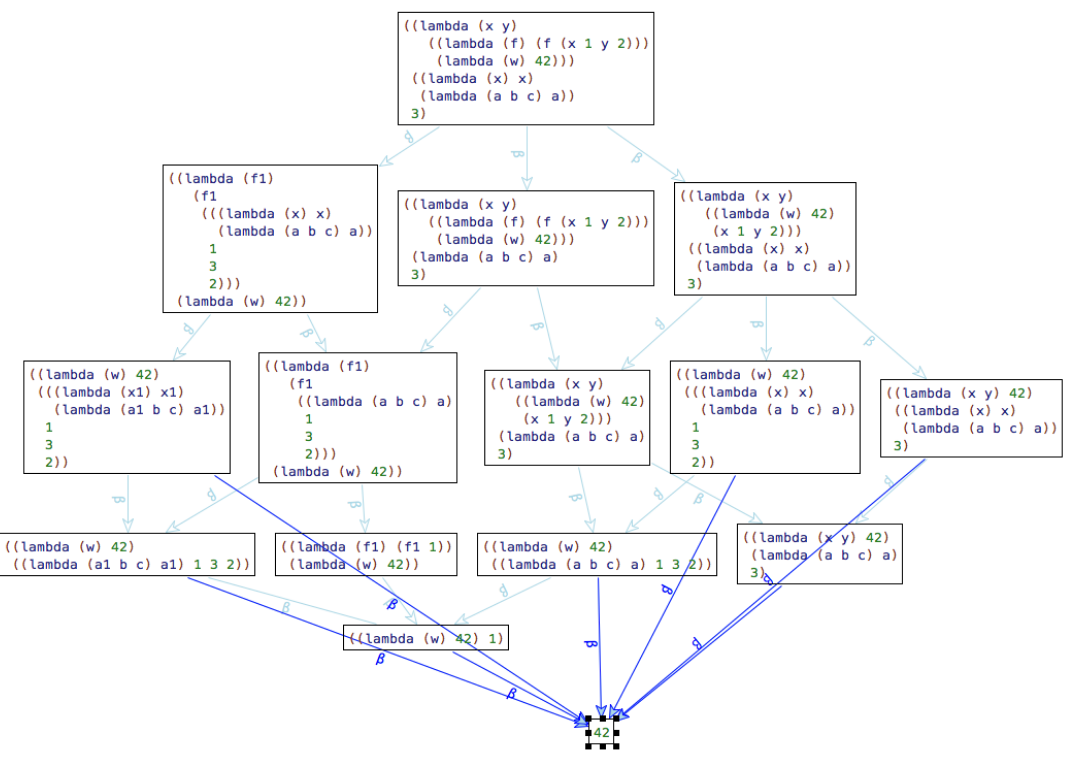
\includegraphics[width=12cm]{images/chapter2/fullbeta.png}
	\caption{完全β规约}
	\label{fig:beta}
\end{figure}

可以看出,在完全β规则中,对任何位置的可β规约的lambda表达式,都可以进行规约。因此,与call-by-name和call-by-value不同的是,这种求值规则是不定序的。

结构化操作语义\cite{structural}之父Gordon Plotkin在1975年的文章\upcite{PLOTKIN}中说明了抽象自动机和递归解释器的表达能力是相同的,而λ演算在一定约束下也具有相同的表达能力,Plotkin的λ演算基于推理规则,如图\ref{fig:plotkin}。

\begin{figure}[ht]
	\centering
	\[\infer {(v~e) → (v~e')}{e~→~e'}  \]
	\[\infer {(e~e'') → (e'~e'')} {e~→~e'}  \]
	\caption{Plotkin's lambda}
	\label{fig:plotkin}
\end{figure} 

	

而1992年Felleisen等人提出的规约语义\upcite{reduction}则是将推理规则优化为了规约规则加上上下文规则,如图\ref{fig:felleisen}的规约语义规则就是和上面两条推理规则等价的。


		\begin{figure}[ht]
			\centering 
			E = (E e) | (v E) | []
			
			if e → e' then E[e] → E[e']
			\caption{Reduction semantic}
			\label{fig:felleisen}
		\end{figure}  


相较于传统的操作语义,规约语义的优点是更容易处理顺序控制和状态信息,本质上属于操作语义,是传统操作语义的一种修订和优化。

PLT Redex\upcite{SEwPR}则是基于规约语义的语言建模工具(也称为语义工程工具),是基于Racket实现的。给定一个语言的文法、上下文规则和规约规则,PLT Redex可以对这个语言的表达式进行规约,生成规约图,随机测试语言正确性等功能。本文运用PLT Redex主要是运用其优秀的语言建模功能。


本文工作的最初思想就是基于完全beta规约。我们在对规约语义不限制上下文环境的情况下,其规约路径也将成为类似完全β规约的图。还是基于上文的例子and(or(\#f, \#t), and(\#t, \#f)),我们可以得到如下的完全规约图\ref{fig:full_reduction}。

\begin{figure}[ht]
	\centering
	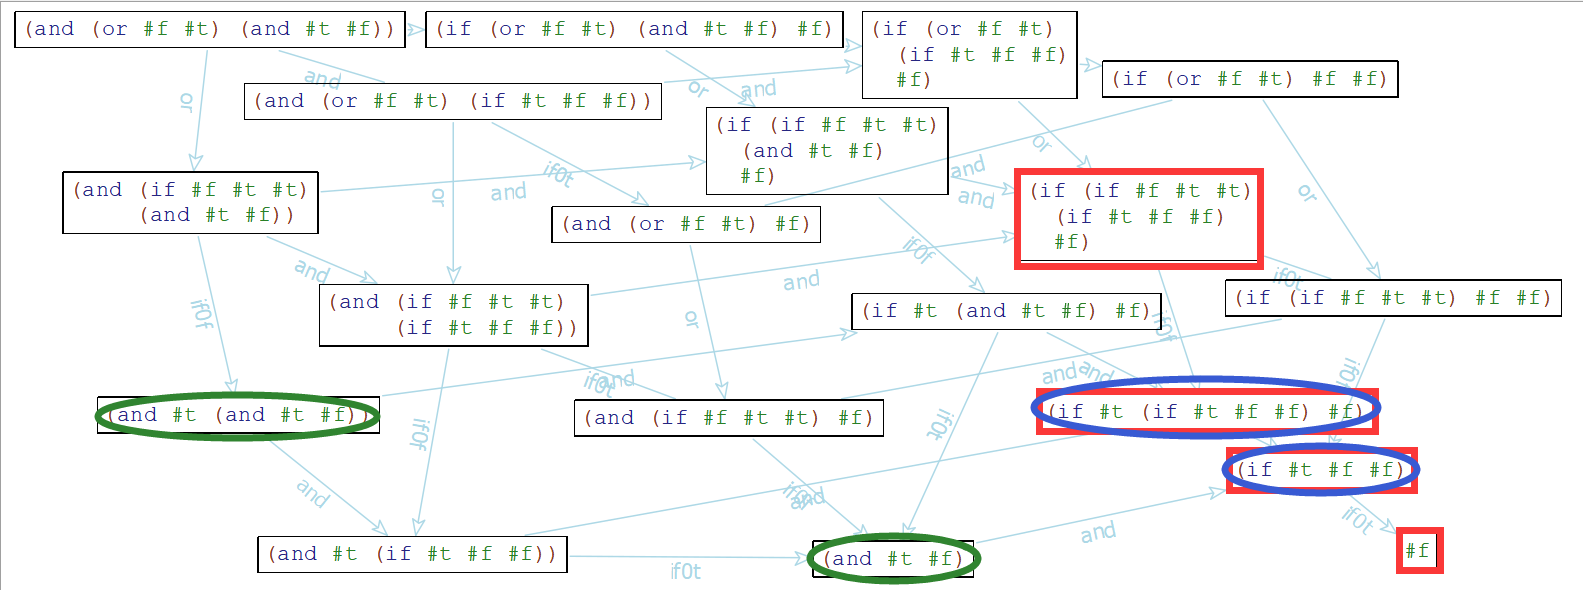
\includegraphics[width=14cm]{images/chapter2/fullreduction.png}
	\caption{完全规约}
	\label{fig:full_reduction}
\end{figure}

在这个图中,我们可以看出,用{\color[rgb]{1,0,0}红色}标出的子序列是将语法糖直接展开后进行规约的求值序列,而这其中有许多中间表达式是可以重组成语法糖的,用{\color[rgb]{0,0,1}蓝色}标出。我们可以发现,在这个中间表达式中可重组的部分就是图\ref{fig:example}中的重组糖序列。而又可以在图中找到{\color[rgb]{0,1,0}绿色}标出的序列---可以惊喜而又自然的发现这一条规约规约路径包含了我们想要的重组糖序列。自然是因为我们对语法糖的规约做了类似完全β规约的处理,导致每个子表达式都有可能首先被规约处理,因此重组糖序列一定在我们的完全图中。

